\chaptr{Anexos}{anexos}

% ----------------------------------------------------------------------------------------------- %

\sect{Anexo A: Pila del producto}{anexoA}

Durante el desarrollo del proyecto se han realizado una serie de tareas, para las cuales se ha utilizado la
herramienta \boldFont{Notion}.
Esta herramienta proporciona una interfaz muy sencilla para la creación de tareas, con la
posibilidad de añadir etiquetas, asignar responsables, añadir comentarios a cada una de ellas,
entre otras funcionalidades.
A continuación, se incluye el fichero pdf generado por Notion con la pila del producto completa.\ Además, se puede
consultar la pila del producto de una manera más interactiva en el siguiente enlace:
\href{https://scastd00.notion.site/9c59c2812d8b440faa453924fef2f320?v=20f7c2f47dd64574ac57713e8efe2718}
{https://scastd00.notion.site/9c59c2812d8b440faa453924fef2f3
20?v=20f7c2f47dd64574ac57713e8efe2718}

% Generar el pdf a 57% de tamaño para que quepa el ancho de página incluyendo las notas de Notion.
\label{anx:product-backlog-notion}
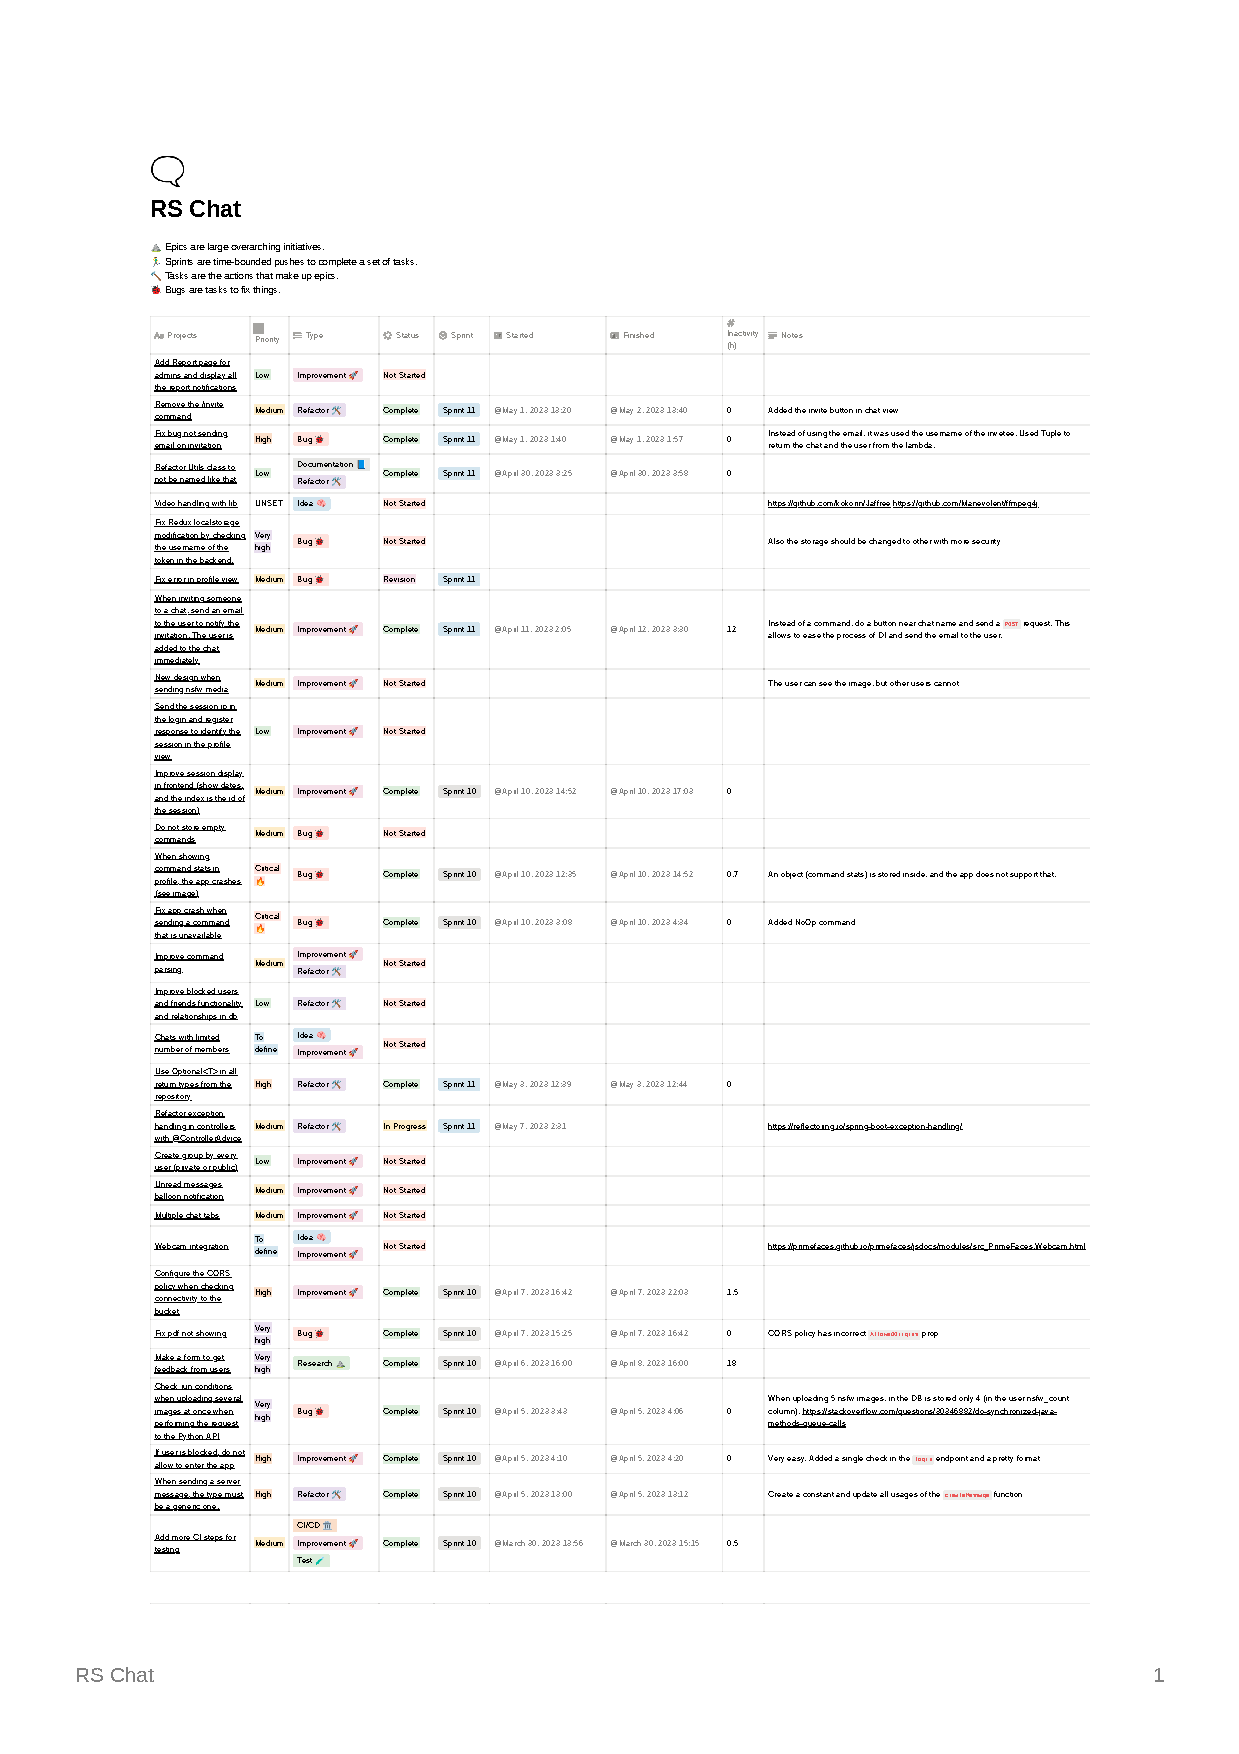
\includepdf[pages=-]{anexos/TareasNotion.pdf}

% ----------------------------------------------------------------------------------------------- %

\sect{Anexo B: Encuesta de satisfacción}{anexoB}

La encuesta de satisfacción realizada a los usuarios se puede visitar en el siguiente enlace:
\href{https://tally.so/r/31XyPQ}{https://tally.so/r/31XyPQ}
\label{anx:encuesta-satisfaccion}

% ----------------------------------------------------------------------------------------------- %

\sect{Anexo C: Diagramas de Gantt}{anexoC}

En esta sección se incluye el diagrama de Gantt completo del proyecto y el enlace a la hoja de cálculo de Google
Sheets con la que se ha generado.\ Además, esta contiene la pila del producto con las tareas completas y los diagramas
de Gantt de cada sprint de manera individual en hojas separadas.\ El enlace a la hoja de cálculo es el siguiente:
\href{https://docs.google.com/spreadsheets/d/1GOffJpsR0vORsQYvTrbWj72jmHIJvB0UMZqahqMcR-s/edit?usp=sharing}
{https://docs.google.com/spreadsheets/d/1GOffJpsR0vORsQYvTrbWj72jmHIJvB0U\\MZqahqMcR-s/edit?usp=sharing}

\label{anx:gantt}
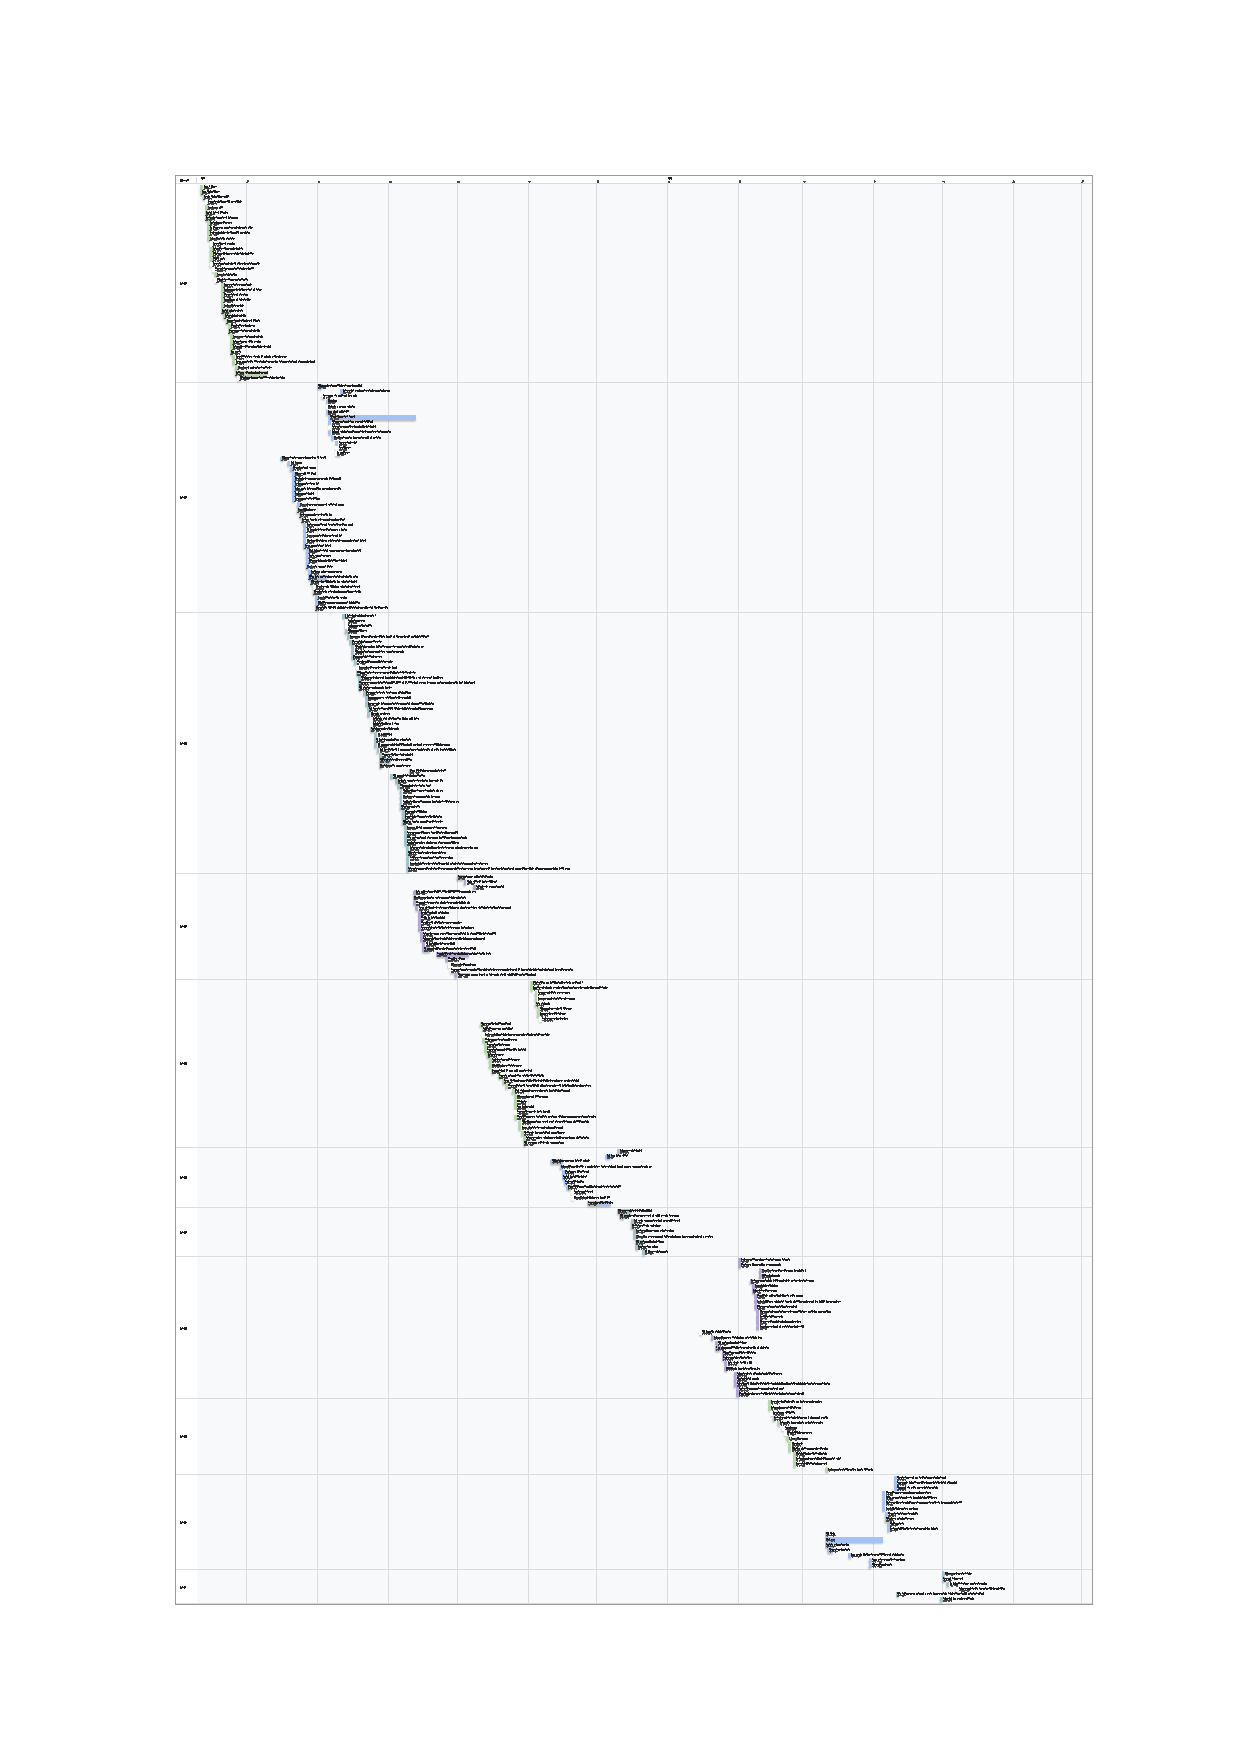
\includepdf[pages=-]{anexos/TodosLosSprints.pdf}

% ----------------------------------------------------------------------------------------------- %

\sect{Anexo D: Política de privacidad}{anexoD}
\label{anx:politica-privacidad-proteccion-datos}

Para garantizar la seguridad de los datos de los usuarios, se ha redactado una política de privacidad
que se puede consultar en el enlace \href{https://rschat.vercel.app/privacy}{https://rschat.vercel.app/privacy}.

De manera resumida, se puede decir que los datos de los usuarios se almacenan en la base de datos alojada en el
servidor local y que no se comparten con terceros.\ Los únicos datos que se almacenan son los necesarios para el
funcionamiento de la aplicación, como son el nombre de usuario, la contraseña, el correo electrónico y el nombre
completo (pero este último solo se muestra en el perfil del propio usuario y no es visible a los demás).\ Además, se
almacena la fecha de última conexión del usuario, para determinar si la sesión actual ha caducado o no.

Todos los usuarios tienen el derecho a solicitar la eliminación de sus datos de la base de datos así como
la eliminación de su cuenta de usuario.\ Para ello, se deberá enviar un correo electrónico a la dirección
\href{mailto:rschat.info@gmail.com}{rschat.info@gmail.com} con el asunto ``Solicitud de eliminación de datos'' y se
procederá a eliminar todos los datos del usuario que el mismo solicite.
